%%Beamer theme "FIUBA", version 0
%%Copyright Luis Gómez
%%22 sep 2023. distributed under the GNU GPL Licence.

%\documentclass{beamer}
\documentclass[aspectratio=169]{beamer}
\usepackage[utf8]{inputenc}
\usepackage[T1]{fontenc} 
%\usepackage[spanish]{babel} 
\usepackage{graphicx}
\usepackage{comment}
\usepackage{pgf,pgfarrows,pgfnodes,pgfautomata,pgfheaps,pgfshade}
%\usepackage{longtable,multirow,booktabs}
\usepackage{amsmath,amssymb}
\usepackage{colortbl}
\usepackage[english]{babel}
\usepackage{graphicx}
\usepackage{array}
\usepackage{multirow}
\usepackage{longtable}
\usepackage{wrapfig}

\usepackage{hyperref}
\usepackage{tcolorbox, empheq}
\usepackage{varwidth}
\usepackage{tikz,tkz-tab}
\usepackage{tikz}
\usetikzlibrary{positioning, arrows.meta, backgrounds, fit}
\usepackage{pgfgantt}
\usepackage{tabularx}
\usepackage{fontawesome5}

\RequirePackage{etoolbox}
\RequirePackage{xparse}



\usetikzlibrary{matrix,arrows, positioning,shadows,shadings,backgrounds, calc, shapes, tikzmark}
\tcbuselibrary{skins,breakable,listings,theorems}


\graphicspath{{images/}}

% % % % % % % % % % % % % % % % % % % %
\usepackage{listings}
\lstset{ frame=Ltb,
framerule=0pt,
aboveskip=0.5cm,
framextopmargin=3pt,
framexbottommargin=3pt,
framexleftmargin=0.2cm,
framesep=0pt,
rulesep=10pt,
%backgroundcolor=\color{gray97},
rulesepcolor=\color{black},
%
stringstyle=\ttfamily,
showstringspaces = false,
basicstyle=\small\ttfamily,
commentstyle=\color{gray45},
keywordstyle=\bfseries,
%
numbers=left,
numbersep=15pt,
numberstyle=\tiny,
numberfirstline = false,
breaklines=true,
}

% minimizar fragmentado de listados
\lstnewenvironment{listing}[1][]
{\lstset{#1}\pagebreak[0]}{\pagebreak[0]}

\lstdefinestyle{consola}
{basicstyle=\scriptsize\bf\ttfamily,
backgroundcolor=\color{gray75},
}

\lstdefinestyle{C}
{language=C,
}



% % % % % % % % % % % % % % % %

\tcbset{opteqA/.style={ %
tcbox
raise base,
nobeforeafter,
extrude by=-2mm,
158
colback=red!50!black!30,
colframe=red!50!black!20}}


% %
% Teal	Light Teal	Orange	Yellow	Brown
% #00878F	#62AEB2	#E47128	#E5AD24	#8C7965


%%Defining the ``proposition'' environment
% %
\definecolor{gris}{rgb}{0.95,0.95,0.95}
\definecolor{verde}{rgb}{0.74,0.75,0.0}
\definecolor{verdeoscuro}{rgb}{0.51,0.52,0.0}
\definecolor{tipsColor}{RGB}{142, 68, 173}
\definecolor{blanco}{RGB}{0, 0, 0}

\newtcolorbox[auto counter, number within=section]{cuadro}[2][]
{ %
	enhanced jigsaw,
	borderline west={1pt}{1pt}{verdeoscuro},
	sharp corners,
	boxrule=1pt,
	fonttitle={\small\bfseries},
	coltitle={white},
	title={\textcolor{tipsColor}{\huge\faLightbulbO} Tip\\},
	%attach title to upper,
	right=0pt,
	top=0pt,
	bottom=0pt,
	frame hidden,
	fonttitle=\bfseries\sffamily\small,
	colbacktitle=verdeoscuro,
	colframe=verdeoscuro,
	colback=gray!5!white, % Color del fondo
	enhanced, width=11cm,
	%attach boxed title to top center={yahift=-2mm}
	title={\thetcbcounter:  #2},#1}


\newtheorem{proposition}{Proposition} 


%%Sets the beamer theme "Cuerna"

\usetheme{FIUBA} 
\usecolortheme{FIUBA}
\useoutertheme{FIUBA}

%\usetheme{Cuerna} 
%\usecolortheme{brick}
%\useoutertheme{infolines}
%Available color themes: default, bluesimplex, brick, lettuce

	\definecolor{GreenColor}{rgb}{0.0, 1.0, 0.0} % Definir color verde
\definecolor{LightRed}{rgb}{1.0, 0.6, 0.6} % Definir color rojo suave
\definecolor{RedColor}{rgb}{1.0, 0.0, 0.0} % Definir color rojo
\definecolor{GreenColor}{HTML}{00FF00}
\definecolor{LightRed}{HTML}{FF6666}
\definecolor{RedColor}{HTML}{FF0000}

\newcommand{\colorcell}[1]{%
	\ifnum#1<10 \cellcolor{GreenColor}%
	\else\ifnum#1<20 \cellcolor{GreenColor!50}%
	\else\ifnum#1<30 \cellcolor{GreenColor!30}%
	\else\ifnum#1<40 \cellcolor{LightRed}%
	\else\ifnum#1<50 \cellcolor{RedColor!50}%
	\else\ifnum#1<60 \cellcolor{RedColor!60}%
	\else\ifnum#1<70 \cellcolor{RedColor!70}%
	\else\ifnum#1<80 \cellcolor{RedColor!80}%
	\else\ifnum#1<90 \cellcolor{RedColor!90}%
	\else \cellcolor{RedColor}%
	\fi\fi\fi\fi\fi\fi\fi\fi\fi
	#1%
}

%%Insert the logo
\logo{\includegraphics[width=2cm]{./logo/logoFIUBA}}

%%Title
%%Title
\title[]{Medidor de material particulado fino }

\author{Autor: Mg. Luis Alberto Gómez Parada\\
Director:  Ing. Juan Manuel Cruz\\ \texttt{correo: lgomez@patagones.cl}} %e-mail
	      
\date{Carrera de Especialización en Sistemas Embebidos} %Date or event

\institute{} %%Institution


\setbeamertemplate{footline}[frame number]


\begin{document}
	
	
	
	
\setbeamertemplate{footline}{}
\begin{frame}

  \titlepage %Creates the title page
  
\end{frame}

%--------------------------------------------------------------------------
\begin{frame}
\tableofcontents %Prints the table of contents
\end{frame}
%--------------------------------------------------------------------------

\section{Introducción}
\setbeamertemplate{footline}[frame number]
\begin{frame}
	\frametitle{Introducción}
	\begin{itemize}
			\item La contaminación atmosférica por MP2,5 se cuenta entre las principales causas de muertes prematuras en el mundo. 
			
		\item Los instrumentos para medir el material particulado fino (MP2,5) son herramientas esenciales para gestionar la calidad de aire de entornos urbanos. 
		\item Sin embargo, lograr una medición precisa es un desafío significativo debido a los elevados costos y los complejos requisitos técnicos.
		\end{itemize} 
	
	\begin{figure}
	\centering
	\includegraphics[width=0.5\linewidth]{images/filtro}
	\caption{Día contaminado en la ciudad de Coyhaique fuente: interne}
	\label{fig:proceso-computacion-fisica}
\end{figure}

\end{frame}

\section{Interesados}

\begin{frame}
	\frametitle{Interesados}

\begin{description}	
\item [Cliente:] instituciones científicas públicas y privadas; gobiernos locales, como municipios y gobiernos regionales; agencias ambientales y ministerios de medio ambiente nacionales.
\item [Usuario final:] corresponde a la población urbana expuesta a episodios de contaminación atmosférica relacionados con MP2,5.
\item [Director:] ingeniero electrónico con amplia experiencia. Su contribución será fundamental en el diseño de la placa electrónica que soportará el instrumental y en la optimización de la programación.
\end{description}	
	\begin{figure}
		\centering
		\includegraphics[width=0.5\linewidth]{images/calidadaire}
		\caption{filtro expuesto en Coyhaique}
		\label{fig:proceso-computacion-fisica}
	\end{figure}
	
	
\end{frame}

\section{Propósito}

\begin{frame}
	\frametitle{Propósito}
	\begin{itemize}
			\item Desarrollar un equipo de medición de material particulado fino (MP2,5) que brinde una mayor precisión y exactitud que los sensores ópticos de bajo costo, mediante técnicas estadísticas de muestreo.
			
			\item Se busca elaborar una solución económica y fiable que pueda integrarse en las redes de control de calidad del aire. 
		\end{itemize}
			
				
			\begin{figure}[htpb]
				\centering
				%\shorthandoff{<>} % Desactivar caracteres problemáticos
				\begin{tikzpicture}[ node distance=0.5cm]
				% Nodes
				\node (microcontroller) 
				[draw, rectangle, fill=blue!10!white, align=center] 						
				{\textbf{Microcontrolador}\\ \rotatebox{90}{\faMicrochip}};  
				
				\node (sensor1) 		
				[above right=of microcontroller, draw, rectangle, fill=red!10!white, align=center, yshift=0.2cm, xshift=0.3cm] 	
				{Sensor de\\MP2,5 \faSmog};
				
				\node (sensor2) 		
				[right=of microcontroller, draw, rectangle, fill=red!10!white, align=center] 		
				{Sensor de\\MP2,5 \faSmog};
				
				\node (sensor3) 		
				[below right=of microcontroller, draw, rectangle, fill=red!10!white, align=center, , yshift=-0.2cm, xshift=0.3cm] 	
				{Sensor de\\MP2,5 \faSmog};
				
				\node (storage) 		
				[below=of microcontroller, draw, fill=yellow!10!white, rectangle, align=center] 		
				{Sistema de \\ almacenamiento  \faSdCard }; % \faDatabase
				
				\node (transmission) 	
				[above=of microcontroller, draw, rectangle, align=center] 		
				{Sistema de transmi-\\sión de datos  \faSignal};
				
				\node (rtc) 			
				[above left=of microcontroller, draw, rectangle, align=center, yshift=-1.5cm, xshift=-.33cm]  
				{RTC \faClock[regular]};
				
				\node (power) 			
				[below left=of microcontroller, draw, rectangle, align=center,yshift=-0.2cm, xshift=0.0cm] 	
				{Fuente de\\alimentación \faBatteryQuarter};
				
				\node (cabinet) 		[above right=of transmission,  xshift=-6.4cm,yshift=-0.7cm]     {\textbf{Gabinete} \faCloudSunRain};
				
				% Bounding Box
				\begin{scope}[on background layer]
				\node[fill=gray!10,  draw, rectangle, rounded corners, fit=(cabinet) (sensor1) (rtc) (power) (transmission)] {};
				\end{scope}
				
				% Arrows
				\draw[<->] (microcontroller) -- (sensor1);
				\draw[<->] (microcontroller) -- (sensor2);
				\draw[<->] (microcontroller) -- (sensor3);
				\draw[<->] (microcontroller) -- (storage);
				\draw[<->] (microcontroller) -- (transmission);
				\draw[->] (rtc) -- (microcontroller);
				\draw[->] (power) -- (microcontroller);
				\end{tikzpicture}
			%	\shorthandon{<>} % Reactivar caracteres problemáticos
				%\caption{Esquema de bloques del instrumento.}
				\label{fig:diagBloques}
			\end{figure}
				 
	
\end{frame}

\section{Requerimientos}

\begin{frame}
	\frametitle{Requerimientos}
		\textbf{Funcionales:}
		\begin{enumerate}
			\item Tres sensores incorporados a la medición de MP2,5.
			\item Las mediciones deben contar tiempo proporcionado por un RTC.
		
		\end{enumerate}
		\textbf{Hardware y energéticos:}
		\begin{enumerate}
			\item La placa de desarrollo debe permitir conectar múltiples sensores.
				\item Fuente de energía compatible con 220 V CA y una batería recargable.
			\item El gabinete de acuerdo a la norma protección IP65. 
				
		\end{enumerate}
		\textbf{Software}
		\begin{enumerate}
			\item Los datos de MP2,5 serán del tipo ``punto flotante".
		\end{enumerate}
		
		\textbf{Interfaz de usuario:}
		\begin{enumerate}
			\item El usuario podrá acceder a los datos históricos medidos por el instrumento.
		\end{enumerate}
		
		\textbf{Evaluación y documentación:}
		\begin{enumerate}
			\item Se realizarán pruebas de calibración con sensores certificados.
			\item Contará con un manual con las características principales del instrumento.
		\end{enumerate}
		
\end{frame}

\section{Alcances}

\begin{frame}
	\frametitle{Alcances del proyecto}
	
	\begin{enumerate}
		\item \textbf{Diseño y desarrollo del hardware}
		\begin{itemize}
			\item Diseño, selección, adquisición y construcción del hardware acorde a los niveles de consumo eléctrico, necesidad de cómputo, almacenamiento y transmisión de datos, necesarios para su funcionamiento.  
		\end{itemize}
		
		\item \textbf{Desarrollo de software}
		\begin{itemize}
			\item Programación del microprocesador para realizar cálculos, validar y transmitir resultados.
		\end{itemize}
		
		\item \textbf{Pruebas de calibración}
		\begin{itemize}
			\item Calibración inicial de los sensores con estaciones de monitoreo de referencia o instrumentos de referencia disponibles.
		\end{itemize}
		
		\item \textbf{Recolección de datos}
		\begin{itemize}
			\item Recolección de datos de MP2,5 para evaluar el funcionamiento y rendimiento del dispositivo.
		\end{itemize}
		
		\item \textbf{Análisis de datos}
		\begin{itemize}
			\item Evaluación de la precisión y exactitud del dispositivo en comparación con los métodos ópticos tradicionales o los de referencia.
		\end{itemize}
		
		\item \textbf{Documentación}
		\begin{itemize}
			\item Generación de informes técnicos que validen el rendimiento y robustez del dispositivo.
		\end{itemize}
		
	\end{enumerate}
	
\end{frame}


\section{Diagrama de Activity On Node}

\begin{frame}
	\frametitle{Diagrama de Activity On Node}
	\centering
	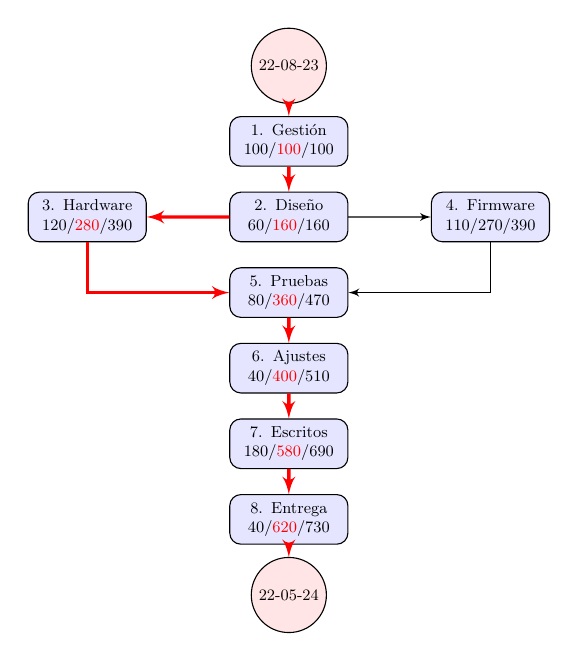
\begin{tikzpicture}[node distance=1.5cm, scale=0.8, every node/.style={scale=0.8, font=\small}, transform shape]
	
	\tikzstyle{block} = [rectangle, draw, fill=blue!10, text width=6em, text centered, rounded corners, minimum height=2.8em]
	\tikzstyle{line} = [draw, -latex']
	\tikzstyle{critical_line} = [draw, red, very thick, -latex']
	\tikzstyle{circleblock} = [circle, draw, fill=red!10, text centered, minimum size=3em]
	
	\node [circleblock, align=center] (init) {22-08-23};
	\node [block, below of=init] (1) {1. Gestión { 100/{\color{red}100}/100}};
	\node [block, below of=1] (2) {2. Diseño { 60/{\color{red}160}/160}};
	\node [block, left of=2, node distance=3cm, xshift=-1cm] (3) {3. Hardware { 120/{\color{red}280}/390}};
	\node [block, right of=2, node distance=3cm, xshift=1cm] (4) {4. Firmware 110/270/390};
	\node [block, below of=2] (5) {5. Pruebas { 80/{\color{red}360}/470}};
	\node [block, below of=5] (6) {6. Ajustes { 40/{\color{red}400}/510}};
	\node [block, below of=6] (7) {7. Escritos { 180/{\color{red}580}/690}};
	\node [block, below of=7] (8) {8. Entrega { 40/{\color{red}620}/730}};
	\node [circleblock, below of=8, align=center] (fin) {22-05-24};
	
	\path [critical_line] (init) -- (1);
	\path [critical_line] (1) -- (2);
	\path [critical_line] (2) -- (3);
	\path [line] (2) -- (4);
	\path [line] (4) |- (5);
	\path [critical_line] (3) |- (5);
	\path [critical_line] (5) -- (6);
	\path [critical_line] (6) -- (7);
	\path [critical_line] (7) -- (8);
	\path [critical_line] (8) -- (fin);
	\end{tikzpicture}
\end{frame}


\section{Carta Gantt}
	\begin{frame}
		\frametitle{Carta Gantt}

			\begin{ganttchart}[
		hgrid,
		vgrid={*4{dotted}, *3{red!50}}, %	vgrid,
		x unit=0.038cm,
		y unit chart=0.5cm,
		time slot format=isodate,
		time slot unit=day,
		bar/.append style={fill=blue!30},
		group/.append style={fill=blue!50},
		%link/.style={->, thick}
		]{2023-09-08}{2024-05-25}
		
		\gantttitlecalendar{year, month} \\
	%	\ganttmilestone{0. Acta de constitución}{2023-09-11}\\
		\ganttgroup{1. Propuesta del proyecto}{2023-09-11}{2023-10-13} \\
	%	\ganttmilestone{1.5 Proyecto de tesis}{2023-10-13} \\
		
		\ganttgroup{2. Diseño general}{2023-10-16}{2023-11-03} \\
		
		\ganttgroup{3. Construcción del HW}{2023-11-06}{2023-12-15} \\
		
		\ganttgroup{4. Construcción del FW}{2023-12-18}{2024-01-24} \\
		
		\ganttgroup{5. Pruebas}{2024-01-24}{2024-02-21} \\

		
		\ganttgroup{6. Ajustes finales}{2024-02-21}{2024-03-06} \\

		\ganttmilestone{Prototipo funcional}{2024-03-06} \\
		
		\ganttgroup{7. Escritura}{2024-03-06}{2024-05-08} \\

	%	\ganttmilestone{Manual técnico}{2024-05-08} \\
		
		\ganttgroup{8. Proceso de cierre}{2024-05-08}{2024-05-22} \\

		\ganttmilestone{Presentación tesis}{2024-05-22}
		
		
	\end{ganttchart}

\end{frame}

\section{Gestión de riesgos}

\begin{frame}
	\frametitle{Gestión de riesgos}
	

 
 	\begin{table}[htpb]
 	
 	\caption{Resumen de la gestión del riesgos con el resultado de las medidas de mitigación.}
 	\label{tab:gestionriesgo}
 	\centering
 	\begin{tabularx}{\linewidth}{|X|c|c|c|c|c|c|}
 		\hline
 		\rowcolor[HTML]{C0C0C0} 
 		Riesgo & S & O & RPN & S* & O* & RPN* \\ \hline
 		Mal funcionamiento de los sensores & 9  & 8  & \colorcell{72}    & 9  & 2  & \colorcell{18}    \\ \hline
 		Autoridades no aceptan mediciones  & 7  & 8  & \colorcell{56}    & 6  & 4  & \colorcell{24}    \\ \hline
 		Fallo en la transmisión de datos   & 6  & 5  & \colorcell{30}    & 2  & 5  & \colorcell{10}     \\ \hline
 		Interrupción de energía            & 8  & 4  & \colorcell{32}    & 6  & 2  & \colorcell{12}     \\ \hline
 		Manipulación o actos de vandalismo    & 8  & 3  & \colorcell{24}    & -  & -  & -     \\ \hline
 		Pérdida de sincronización del RTC  & 7  & 3  & \colorcell{21}    & -  & -  & -     \\ \hline
 	\end{tabularx}%
 \end{table}
 
\end{frame}

\section{Gestión de la calidad}

\begin{frame}
	\frametitle{Gestión de la calidad}
\begin{description}
	
	\item [Req \#01:] exactitud y precisión  para estimar las concentraciones de MP2,5.
	\item [Req \#02:] transmisión de datos segura y sin fallos a la base de datos.
	\item [Req \#03:] sistema de alimentación energética fiable.
	\item [Req \#04:] almacenamiento de datos en el instrumento.
	\item [Req \#05:] datos que cuentan con un índice temporal sincronizado.
	\item [Req \#06:] funcionamiento efectivo del equipo bajo diversas condiciones ambientales. 
	\item [Req \#07:] disponibilidad de un manual de usuario claro.
	\item [Req \#08:] disponibilidad de parámetros básicos de registro  de MP2,5.
	\item [Req \#09:] implementación de buenas prácticas de programación en el software.
	\item [Req \#10:] evaluación de consumos eléctricos y de datos.

\end{description}
\end{frame}
\begin{frame}
	\frametitle{Gestión de la calidad}
	\textbf{Ejemplo:}
	

\begin{description}
	
	\item [Req \#1:] exactitud y precisión del instrumento para estimar las concentraciones atmosféricas de MP2,5.
	
	\begin{description}
		\item [Verificación:] se deben realizar al menos tres pruebas comparativas con el fin de asegurar que los sensores proporcionan medidas de las concentraciones de MP2,5 con la precisión y exactitud requeridas. El éxito se determinará al lograr una precisión y exactitud que se encuentre en un rango aceptable entre los sensores de bajo costo y los métodos de referencia estandarizados. 
		\item [Validación:] los resultados de las pruebas se presentarán al cliente para su evaluación y aprobación,  cumpliendo con sus expectativas y requisitos.
	\end{description}
		 
	\end{description} 

\end{frame}

\section{Cierre}

\begin{frame}
	\frametitle{Proceso de cierre}

\begin{itemize}
		\item Pautas de trabajo para analizar el respeto al Plan de Proyecto original
		\begin{itemize}

			\item \textbf{Procedimiento:} comparar los resultados obtenidos con los objetivos establecidos en el Plan de Proyecto original, documentar desviaciones y analizar sus causas.
			\item \textbf{Registro:} texto que contiene análisis comparativo.
		\end{itemize}
		
		\item Identificación de técnicas y procedimientos y solución de problemas
		\begin{itemize}
	
			\item \textbf{Procedimiento:} celebrar una reunión retrospectiva para discutir y documentar las lecciones aprendidas y los problemas surgidos.
			\item \textbf{Registro:} texto que contiene ``lecciones aprendidas".
		\end{itemize}
		
		\item Acto de agradecimiento
		\begin{itemize}
			
			\item \textbf{Procedimiento:} ceremonia de agradecimiento y entrega de certificados de reconocimiento. En este acto se agradecerá a todas las personas
			que contribuyeron, jurados, docentes, autoridades de la carrera de especialización,
			colegas y autoridades.
		\end{itemize}
		\end{itemize}

\end{frame}


\end{document}


%%%%%%%%%%%%%%%%%%%%%%%%%%%%%%%%%%%




